\chapter{Three Element Control}

As discussed in Section 2.1, PID control is by design not optimized. It is however a proven tool used in industry and has been able to satisfactorily control boilers for decades. This chapter will discuss on the physical dynamics of how the PID control strategy seen in Figure \ref{fig:3_element_control} can be used on the Expanded model in Equation \ref{eq:Valve_Model_1} without linearization. It should be noted that many power plants use adaptive controller gains in conjecture with the three element control stragety. 

   %     $$ x = \left [\begin{matrix} V_{wt} & p & \alpha_r & V_{sd} & Q & q_{fw}\end{matrix} \right]^T$$
   %     $$ u = \left [\begin{matrix}  & FW_{valve} \end{matrix} \right]^T$$  

\section{Controller Design}

    The model in place requires control inputs to the Feed Water Valve and the Fuel Valve. The Fuel valve controls pressure directly, but due to the dynamics of the boiler, level control cannot be decoupled entirely, and the steam flow out becomes part of the three element controller. 
    
    For this design, the Controlers were tuned to be stable, but not optimized. 
    
    The controller for the Pressure is designed as a PI controller with the following gains:
    $$ \begin{matrix} K_p = 100   & & & K_i = 0.15 \end{matrix} $$
    \begin{equation}
        \label{eq:PID_Q_VALVE}
        Q_{valve} = \left( K_p + K_i \frac{1}{s} \right)\left( p_{ref} - p \right)
    \end{equation}
    The Three Element controller follows the format shown in Figure \ref{fig:Alt_3_element_control}. 
    
    The Level Controller has the following Gains:
    $$ \begin{matrix} K_p = 250   & & & K_i = 1 \end{matrix} $$
    \begin{equation}
        \label{eq:PID_FW_SP}
        q_{fw sp} = \left( K_p + K_i \frac{1}{s} \right)\left( l_{ref} - l \right)
    \end{equation}
    
    The Level Controller then feeds into the Feed Water Controller and the Feed Water Controller has a feed Forward. The following gains and equations apply:
    $$ \begin{matrix} K_p = 1 & & & K_i = 1  & & & K_{ff} = 1\end{matrix}$$
    \begin{equation}
        \label{eq:PID_FW_VALVE_1}
        FW_{valve} = \left( K_p + K_i \frac{1}{s} \right)\left( q_{fwsp} - q_{fw} \right) + K_{ff} q_s
    \end{equation}
    
    The cascaded control is then calculated by combining \eqref{eq:PID_FW_SP} and \eqref{eq:PID_FW_VALVE_1} to get \eqref{eq:PID_FW_VALVE}
    \begin{equation}
        \label{eq:PID_FW_VALVE}
        FW_{valve} = \left( K_p + K_i \frac{1}{s} \right)\left( \left( K_p + K_i \frac{1}{s} \right)\left( l_{ref} - l \right) - q_{fw} \right) + K_{ff} q_s
    \end{equation}
    
    These PID Controllers \eqref{eq:PID_Q_VALVE}\eqref{eq:PID_FW_VALVE} were integrated into the Expanded Valve Model seen in Equation \ref{eq:Valve_Model_1}, which increased the number of states by 3 (one for each I term in the PI Controllers). 
    The new state variable for the PID closed loop system is as follows:
    $$\begin{matrix} \left [ \begin{matrix} V_{wt} & p & \alpha_r & V_{sd} & Q_{valve} & FW_{valve} & \left( p_{ref} - p \right) & \left( q_{fwsp} - q_{fw} \right) & \left( l_{ref} - l \right) \end{matrix} \right ]^T \end{matrix}$$

\section{Simulation Results}

    The simulation using the PID can be calculated using the full nonlinear model, with no linearisation required. It should be noted that the chosen gain values may not control properly over a large range. 
    
    Below are Step Responses for changes in the Reference (Set Point) for the Drum Pressure Controller \eqref{eq:PID_Q_VALVE}.
    
    \begin{figure}[ht]
        \begin{center}
            \resizebox{\ScaleMLFigFour \textwidth}{!}{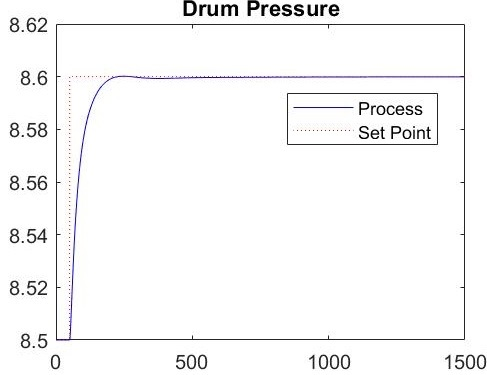
\includegraphics{Controlers/ThreeElement/PressStep/PID1/PID1-3.jpg}}
            \caption{Drum Pressure PID Response to Drum Pressure increase of 0.1}
            \label{fig:PID_Pressure_PressStep}
        \end{center}
    \end{figure}  % Drum Pressure PID     Response to Drum Pressure increase of 0.1  
    \begin{figure}[ht]
        \begin{center}
            \resizebox{\ScaleMLFigFour \textwidth}{!}{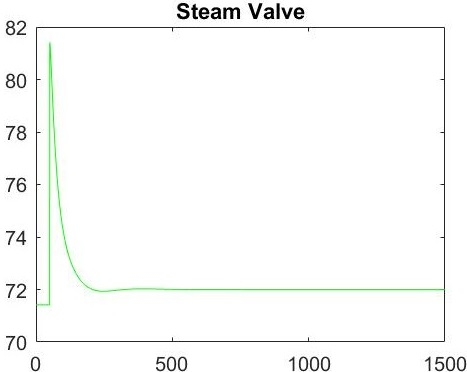
\includegraphics{Controlers/ThreeElement/PressStep/PID1/PID1-6.jpg}}
            \caption{Drum Pressure Control Response $Q_{valve}$ to Drum Pressure increase of 0.1}
            \label{fig:PID_Pressure_PressStep_Control}
        \end{center}
    \end{figure}  % Drum Pressure Control Response to Drum Pressure increase of 0.1     
    
    \begin{figure}[ht]
        \begin{center}
            \resizebox{\ScaleMLFigFour \textwidth}{!}{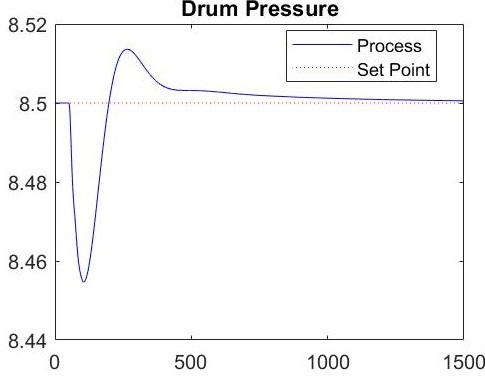
\includegraphics{Controlers/ThreeElement/LvlStep/PID4/PID4-3.jpg}}
            \caption{Drum Pressure PID Response to Level increase of 0.1}
            \label{fig:PID_Pressure_LvlStep}
        \end{center}
    \end{figure}  % Drum Pressure PID Response to Level increase of 0.1    
    \begin{figure}[ht]
        \begin{center}
            \resizebox{\ScaleMLFigFour \textwidth}{!}{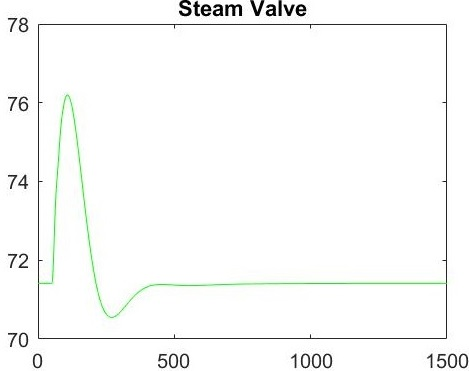
\includegraphics{Controlers/ThreeElement/LvlStep/PID4/PID4-6.jpg}}
            \caption{Drum Pressure Control Response $Q_{valve}$ to Level increase of 0.1}
            \label{fig:PID_Pressure_LvlStep_Control}
        \end{center}
    \end{figure}  % Drum Pressure Control Response to Level increase of 0.1   
    
    Figures \ref{fig:PID_Pressure_PressStep}-\ref{fig:PID_Pressure_LvlStep_Control} show that the model chosen can have pressure adequately controlled by a simple PID. In figure \ref{fig:PID_Pressure_PressStep_Control} it should be noted that a drastic jump in the control is used. This is to be considered heat demand, as $Q_{valve}$ is a simplification of heat addition into the boiler, and the state $Q$ does not have such a drastic curve. Figures \ref{fig:PID_Pressure_PressStep}-\ref{fig:PID_Pressure_PressStep_Control} shows a step response with desirable control settings. Figures \ref{fig:PID_Pressure_LvlStep}-\ref{fig:PID_Pressure_LvlStep_Control} shows a disturbance rejection, as the set point for Drum Pressure never changes. The initial response and long settling time appear as if they can be improved upon.
    
    %% NOTE TO SELF BORZELLIERI BISWAS Search tag: Add in graph for Q vs Q_valve. Reprint PIDs so that it doesn't say Steam valve. That is wrong. 
    
    \clearpage
    
    Below are the Step Responses for the changes in Reference (Set Point) for the \textit{Three Element} Level Controller.
    
    \begin{figure}[ht]
        \begin{center}
            \resizebox{\ScaleMLFigFour \textwidth}{!}{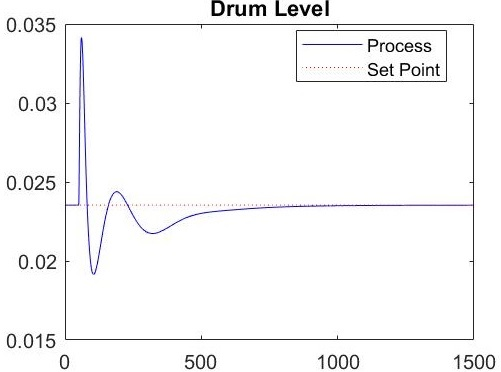
\includegraphics{Controlers/ThreeElement/PressStep/PID1/PID1-2.jpg}}
            \caption{Drum Level PID Response to Drum Pressure increase of 0.1}
            \label{fig:PID_Level_PressStep}
        \end{center}
    \end{figure}   % Drum Level PID Response to  Drum Pressure increase of 0.1
    \begin{figure}[ht]
        \begin{center}
            \resizebox{\ScaleMLFigFour \textwidth}{!}{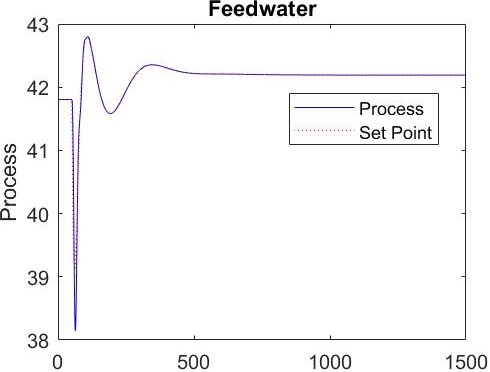
\includegraphics{Controlers/ThreeElement/PressStep/PID1/PID1-1.jpg}}
            \caption{Feedwater PID Response to Cascaded Control Set Point}
            \label{fig:PID_Feedwater_PressStep}
        \end{center}
    \end{figure}   % Feedwater PID Response to Cascaded Control Set Point
    \begin{figure}[ht]
        \begin{center}
            \resizebox{\ScaleMLFigFour \textwidth}{!}{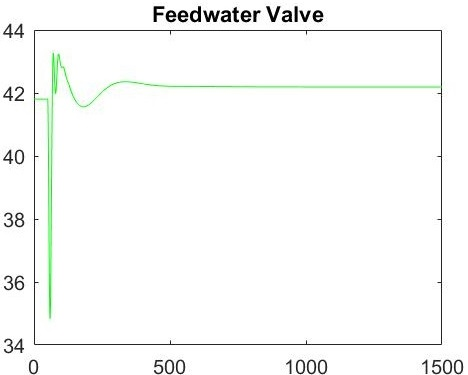
\includegraphics{Controlers/ThreeElement/PressStep/PID1/PID1-4.jpg}}
            \caption{Feedwater Valve and Steam Flow (Feed Forward) to Feedwater Cascaded Control}
            \label{fig:PID_Feedwater_PressStep_Control}    
        \end{center}
    \end{figure}   % Feedwater Valve and Steam Flow (Feed Forward) to Feedwater Cascaded Control
    
    \begin{figure}[ht]
        \begin{center}
            \resizebox{\ScaleMLFigFour \textwidth}{!}{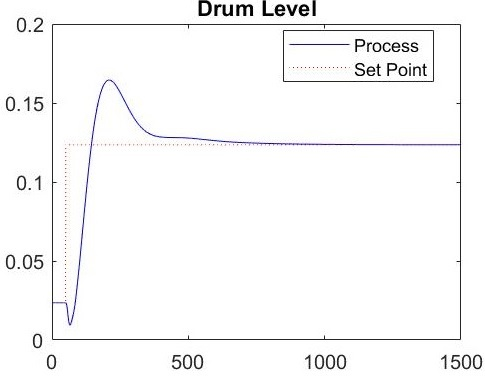
\includegraphics{Controlers/ThreeElement/LvlStep/PID4/PID4-2.jpg}}
            \caption{Drum Level PID Response to a Level increase of 0.1}
            \label{fig:PID_Level_LvlStep}
        \end{center}
    \end{figure}   % Drum Level PID Response to a Level increase of 0.1
    \begin{figure}[ht]
        \begin{center}
            \resizebox{\ScaleMLFigFour \textwidth}{!}{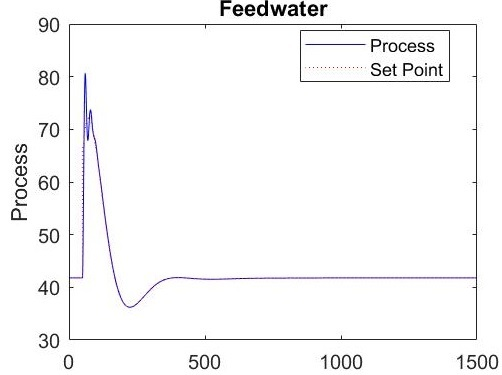
\includegraphics{Controlers/ThreeElement/LvlStep/PID4/PID4-1.jpg}}
            \caption{Feedwater PID Response to Cascaded Control Set Point}
            \label{fig:PID_Feedwater_LvlStep}
        \end{center}
    \end{figure}   % Feedwater PID Response to Cascaded Control Set Point
    \begin{figure}[ht]
        \begin{center}
            \resizebox{\ScaleMLFigFour \textwidth}{!}{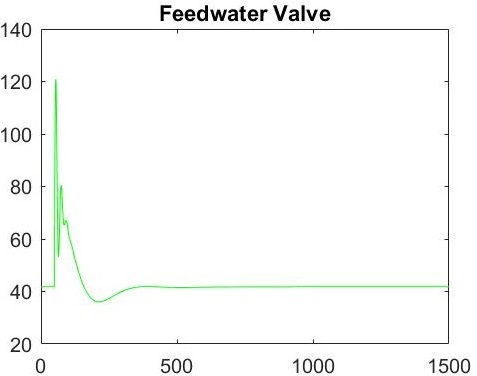
\includegraphics{Controlers/ThreeElement/LvlStep/PID4/PID4-4.jpg}}
            \caption{Feedwater Valve and Steam Flow (Feed Forward) to Feedwater Cascaded Control}
            \label{fig:PID_Feedwater_LvlStep_Control} 
        \end{center}
    \end{figure}   % Feedwater Valve and Steam Flow (Feed Forward) to Feedwater Cascaded Control
    
    Figures \ref{fig:PID_Level_PressStep}-\ref{fig:PID_Feedwater_LvlStep_Control} show that the model chosen can have drum level adequately controlled by the three element control strategy used in industry. Figures \ref{fig:PID_Level_LvlStep}-\ref{fig:PID_Feedwater_LvlStep_Control} shows a step response in terms of level, as the Drum Level set point increases by 0.1. Note the inner loop of Feedwater Flow has its set point change drastically to maintain level. Figures \ref{fig:PID_Level_PressStep}-\ref{fig:PID_Feedwater_PressStep_Control} shows a disturbance response in terms of level, as the Drum Level set point stays constant. Note the inner loop of Feedwater Flow has its set point change drastically to maintain level. Figures \ref{fig:PID_Level_PressStep} \& \ref{fig:PID_Level_LvlStep} show the controller output for the level controller. The controller output for these loops is a set point for the inner cascade loop, and can be see on figures \ref{fig:PID_Feedwater_PressStep} \& \ref{fig:PID_Feedwater_PressStep_Control}. Figures \ref{fig:PID_Feedwater_PressStep} \& \ref{fig:PID_Feedwater_LvlStep} show the tracking response of the inner cascade controller for Feedwater, and Figures \ref{fig:PID_Feedwater_PressStep_Control} \& \ref{fig:PID_Feedwater_LvlStep_Control} show the controller output. Figures \ref{fig:PID_Feedwater_PressStep_Control} \& \ref{fig:PID_Feedwater_LvlStep_Control} also show steam flow, as it is a feed forward to the controller. 
    
    %% NOTE TO SELF BORZELLIERI BISWAS (Search tags): Update Graphics to show Feedwater Valve and Steam Flow, and Feedwater SP vs Feedwater Flow. 